\documentclass{standalone}
\usepackage{graphicx}	
\usepackage{amssymb, amsmath}
\usepackage{color}

\usepackage{tikz}
\usetikzlibrary{intersections, backgrounds, math}
\usepackage{pgfmath}

\definecolor{light}{RGB}{220, 188, 188}
\definecolor{mid}{RGB}{185, 124, 124}
\definecolor{dark}{RGB}{143, 39, 39}
\definecolor{highlight}{RGB}{180, 31, 180}
\definecolor{light_teal}{RGB}{107, 142, 142}
\definecolor{mid_teal}{RGB}{72, 117, 117}
\definecolor{dark_teal}{RGB}{29, 79, 79}
\definecolor{gray10}{gray}{0.1}
\definecolor{gray20}{gray}{0.2}
\definecolor{gray30}{gray}{0.3}
\definecolor{gray40}{gray}{0.4}
\definecolor{gray60}{gray}{0.6}
\definecolor{gray70}{gray}{0.7}
\definecolor{gray80}{gray}{0.8}
\definecolor{gray90}{gray}{0.9}
\definecolor{gray95}{gray}{0.95}

\begin{document}

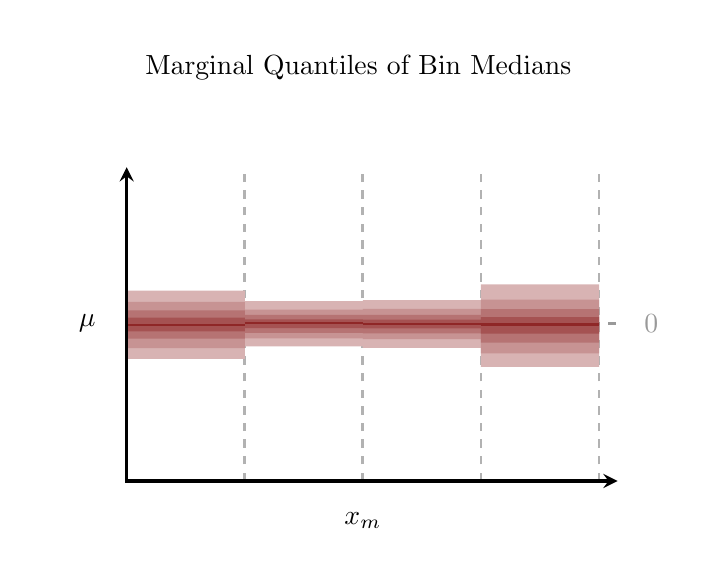
\begin{tikzpicture}[scale=1.0]

  \begin{scope}[shift={(8.5, -6.75)}]
    \draw[white] (-4.25, -3) rectangle (4.25, 3.75);
    
    \node[align=center] at (0, 3.25) { Marginal Quantiles of Bin Medians };
    
    \foreach \b in {-3.0, -1.5,  0.0,  1.5,  3.0} {
      \draw[gray70, dashed, line width=1] (\b, -2) -- (\b, 2);
    }
    
    \draw[gray60, dashed, line width=1] (-3, 0) -- (3.25, 0);   
    \node[gray60, anchor=west] at (3.1, 0)  { $\quad 0$ };
    
    \foreach \a/\b/\c/\d/\e/\f/\g/\h [count=\n] in {-0.449/-0.291/-0.310/-0.551/0.498/0.297/0.284/0.418,
                                                    -0.312/-0.190/-0.198/-0.378/0.302/0.187/0.177/0.275,
                                                    -0.193/-0.118/-0.124/-0.243/0.183/0.111/0.110/0.166,
                                                    -0.099/-0.060/-0.063/-0.127/0.082/0.048/0.054/0.076} {
       \pgfmathsetmacro{\prop}{20 + 15 * \n};
       \colorlet{custom}{dark!\prop!white};
       \fill[custom] (-3, \a) -- (-1.5, \a) --
                     (-1.5, \b) -- (0, \b) --
                     (0, \c) -- (1.5, \c) --
                     (1.5, \d) -- (3, \d) --
                     (3, \e) -- (1.5, \e) --
                     (1.5, \f) -- (0, \f) --
                     (0, \g) -- (-1.5, \g) --
                     (-1.5, \h) -- (-3, \h) -- cycle;
    }
    
    \foreach \a/\b/\c/\d in {-0.018364718/0.005751360/-0.006619488/-0.017072498} {
      \draw[dark, line width=1] (-3, \a) -- (-1.5, \a);
      \draw[dark, line width=1] (-1.5, \b) -- (0, \b);
      \draw[dark, line width=1] (0, \c) -- (1.5, \c);
      \draw[dark, line width=1] (1.5, \d) -- (3, \d);
    }
     
    \draw [->, >=stealth, line width=1.25] (-3.00, -2.015) -- +(0, 4);
    \draw [->, >=stealth, line width=1.25] (-3.015, -2.00) -- +(6.25, 0);
    
    \node at (-3.5, 0) { $\mu$ };
    \node at (0, -2.5) { $x_{m}$ };
  \end{scope}
  
\end{tikzpicture}

\end{document}  